% !TeX program = pdflatex
\documentclass[11pt,a4paper]{article}

% Essential packages
\usepackage[utf8]{inputenc}
\usepackage[T1]{fontenc}
% \usepackage[sort&compress]{natbib} % Commented out for debugging
\usepackage{amsmath}
\usepackage{amsfonts}
\usepackage{amssymb}
\usepackage{graphicx}
\usepackage{hyperref}
\usepackage{geometry}
\usepackage{setspace}
\usepackage{booktabs}
\usepackage{float}
\usepackage{cleveref}
\usepackage{titling}
\usepackage{xcolor}
\usepackage{tikz}
\usepackage{fancyhdr}
\usetikzlibrary{shapes,arrows,positioning,decorations.pathreplacing}
\usepackage{caption}
\captionsetup{skip=0pt}  % Remove space between figure and caption

% Define custom colors for Plutchik's Wheel (Primary, Secondary, Tertiary)
% % Primary Emotions (8) % COMMENTING OUT STARTS HERE
% \definecolor{myJoyColor}{RGB}{255,215,0}    % Gold (Joy)
% \definecolor{myTrustColor}{RGB}{0,139,139}  % DarkCyan (Trust)
% \definecolor{myFearColor}{RGB}{139,0,139}   % DarkMagenta (Fear)
% \definecolor{mySurpriseColor}{RGB}{255,140,0} % DarkOrange (Surprise)
% \definecolor{mySadnessColor}{RGB}{65,105,225} % RoyalBlue (Sadness)
% \definecolor{myDisgustColor}{RGB}{0,100,0}   % DarkGreen (Disgust)
% \definecolor{myAngerColor}{RGB}{220,20,60}   % Crimson (Anger)
% \definecolor{myAnticipationColor}{RGB}{255,140,0} % DarkOrange (Anticipation, same as Surprise)

% Secondary Emotions (Dyads - 8)
\definecolor{myOptimismColor}{RGB}{255,179,71} % Apricot (Anticipation+Joy)
\definecolor{myLoveColor}{RGB}{255,105,180} % HotPink (Joy+Trust)
\definecolor{mySubmissionColor}{RGB}{173,216,230} % LightBlue (Trust+Fear)
\definecolor{myAweColor}{RGB}{221,160,221} % Plum (Fear+Surprise)
\definecolor{myDisapprovalColor}{RGB}{250,128,114} % LightCoral (Surprise+Sadness)
\definecolor{myRemorseColor}{RGB}{100,149,237} % CornflowerBlue (Sadness+Disgust)
\definecolor{myContemptColor}{RGB}{189,183,107} % DarkKhaki (Disgust+Anger)
\definecolor{myAggressivenessColor}{RGB}{255,99,71} % Tomato (Anger+Anticipation)

% Tertiary Emotions (8)
\definecolor{myDelightColor}{RGB}{255,223,0} % Brighter Gold (Joy + Love)
\definecolor{myObedienceColor}{RGB}{176,224,230} % PowderBlue (Trust + Submission)
\definecolor{myTerrorColor}{RGB}{230,190,255} % Lavender (Fear + Awe)
\definecolor{myAlarmColor}{RGB}{255,182,193} % LightPink (Surprise + Disapproval)
\definecolor{myDespairColor}{RGB}{119,136,153} % LightSlateGray (Sadness + Remorse)
\definecolor{myShameColor}{RGB}{210,180,140} % Tan (Disgust + Contempt)
\definecolor{myFuryColor}{RGB}{255,69,0}   % OrangeRed (Anger + Aggressiveness)
\definecolor{myHopeColor}{RGB}{255,200,0} % Lighter/Brighter Gold (Anticipation + Optimism)

% Page layout
\geometry{
    a4paper,
    margin=2.5cm
}

% Hyperref settings
\hypersetup{
    colorlinks=true,
    linkcolor=blue,
    filecolor=magenta,
    urlcolor=cyan,
    citecolor=blue
}

% Document info
\title{Songjam\\[0.5em]\large A Cryptographic Voice Verification Network}
\author{Adam Place}
\date{\today}

% Customize title formatting
\pretitle{\begin{center}\LARGE\bfseries}
\posttitle{\par\end{center}}

\begin{document}

\maketitle
\thispagestyle{fancy} % Apply fancy style to the title page
\pagestyle{fancy}
\fancyhf{} % Clear all header and footer fields
\fancyfoot[L]{\thepage} % Page number on the left
\fancyfoot[R]{\small v 0.2} % Version number on the right
\renewcommand{\headrulewidth}{0pt} % No header rule
\renewcommand{\footrulewidth}{0.4pt} % Footer rule

\begin{abstract}
A fully encrypted, privacy-preserving voice verification network could effectively eliminate voice-based deepfake fraud without requiring users to compromise their security or personal data.
Zero-knowledge proofs provide part of the solution, but a fundamental challenge remains: it is difficult to absolutely verify that a given voice truly belongs to a specific individual, especially as voice synthesising technology becomes increasingly sophisticated.
This work introduces a solution to the verification problem by leveraging cryptoeconomics.
Leveraging the security of a Proof-of-Stake (PoS) consensus mechanism, and an open-source hardware system to couple vocal biosignal verification with voice audio.
Cryptographic keys to voice biometrics and other sensitive data are derived from Trusted Execution Environments (TEEs) providing hardware-backed isolation.
Access to these keys is granted to users through a consensual proto-Soulbound Token (SBT), a non-transferable, non-replicable digital asset tied to an individual's digital identity \cite{buterin2022soulbound}.
Over time, the user builds-up a personalised voice model, with each new audio sample organised and stored within a WavRAG structure---an Audio-Integrated Retrieval Augmented Generation framework, enabling efficient and context-rich retrieval of voice data \cite{chen2025wavrag}.
\end{abstract}

\section{Introduction}
\label{sec:introduction}
The rise of deepfakes has led to a growing concern about the fallibility of humans to verify the authenticity of voice communication.
High profile cases such as the 2024 deepfake attack on engineering firm Arup, which led to a twenty-five million dollar loss, highlight the importance of secure and reliable enterprise verification systems.

While a plethora of fraudulent online videos featuring deepfakes of celebrities promoting supposed investment opportunities, and the rise of romance or \textquotesingle pig butchering\textquotesingle{} scams which collectively siphon billions of dollars from unsuspecting victims every year illustrate the necessity of consumer or citizen protections \cite{economist2024scaminc}.
The sub-150ms latency required for natural conversation in VoIP calls leaves minimal time for analysis on standard hardware, making real-time detection of deepfakes challenging. While the proprietary nature of platforms such as Zoom, Teams and SIP providers, hinders the development of universal detection frameworks.

What is needed is a privacy-preserving verification system leveraging zero-knowledge proofs and selective disclosure mechanisms, where only cryptographically attested credentials (e.g., identity, access rights) are validated—without exposing extraneous user data.
This approach ensures networks authenticate voice participants a priori through mathematical guarantees (e.g., zk-SNARKs), verifying the existence of valid credentials rather than analysing raw biometrics or personal details.
By limiting verification to key attributes (e.g., "member of authorised group" or "registered device") and eliminating unnecessary data collection, such systems support user control over personal information while thwarting deepfake fraud and metadata misuse.
This paper proposes a novel cryptoeconomic framework for voice verification, in which users are incentivised to provide accurate and verifiable credentials, while malicious actors face penalties—PoS slashing mechanisms—for fraudulent voice attribution attempts.

\section{The Proof-of-Stake Security Guarantee?}
\label{sec:background}
Much has been written about the security of the PoS consensus mechanism, with proponents arguing that its economic incentives guarantee security, while opponents contend that the consolidation of staked token supply will lead to centralisation.
Nevertheless, the economic incentives and penalties underpinning Ethereum's Proof-of-Stake mechanism have proven effective, driving its adoption and establishing it as the preferred consensus model for securing one of the world's largest blockchain networks—demonstrated by the very small number of validator slashing events recorded to date (with under 0.04\% of validators slashed since Ethereum staking began) \cite{consensys2024slashing}.

\begin{figure}[H]
    \centering
    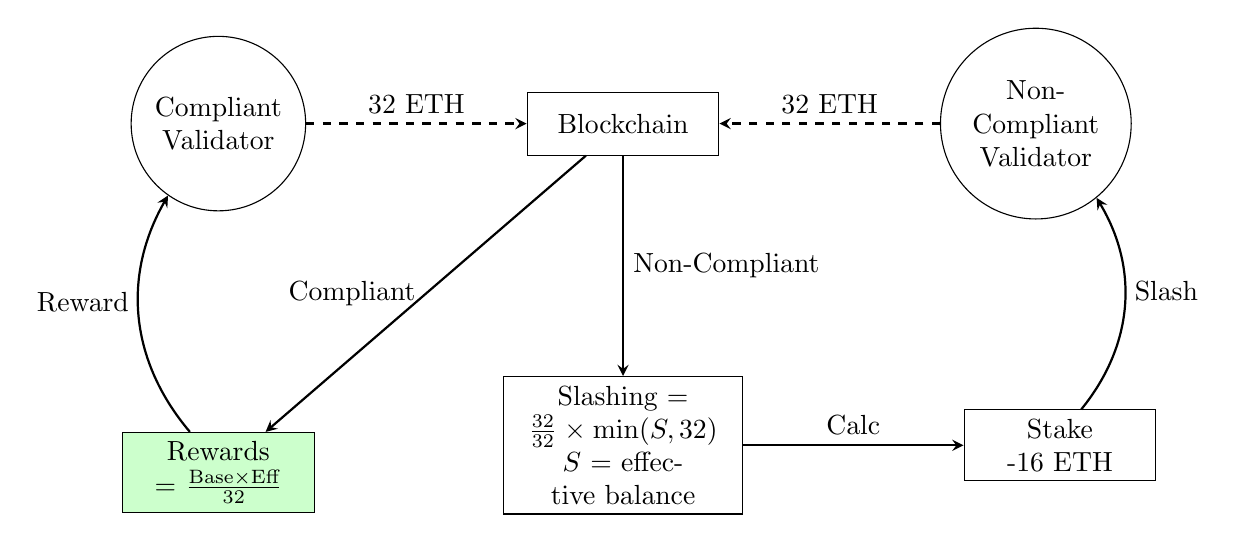
\begin{tikzpicture}[
        node distance=2.8cm,
        block/.style={rectangle, draw, text width=2.2cm, text centered, minimum height=0.8cm},
        validator/.style={circle, draw, text width=1.8cm, text centered, minimum height=0.8cm},
        arrow/.style={thick,->,>=stealth},
        dashedarrow/.style={thick,dashed,->,>=stealth},
        math/.style={rectangle, draw, text width=2.8cm, text centered, minimum height=1.2cm},
        reward/.style={rectangle, draw, text width=2.2cm, text centered, minimum height=0.8cm, fill=green!20}
    ]
        % Blockchain
        \node[block] (blockchain) {Blockchain};
        
        % Validators - using larger distances
        \node[validator, left=2.8cm of blockchain] (validator1) {Compliant Validator};
        \node[validator, right=2.8cm of blockchain] (validator2) {Non-Compliant Validator};
        
        % Staking connections
        \draw[dashedarrow] (validator1) -- node[above] {32 ETH} (blockchain);
        \draw[dashedarrow] (validator2) -- node[above] {32 ETH} (blockchain);
        
        % Slashing penalty
        \node[math, below=of blockchain] (penalties) {
            Slashing = $\frac{32}{32} \times \text{min}(S, 32)$\\
            $S$ = effective balance
        };
        
        % Stake reduction
        \node[block, right=of penalties] (reduction) {Stake -16 ETH};
        
        % Rewards
        \node[reward, below=of validator1] (rewards) {
            Rewards = $\frac{\text{Base} \times \text{Eff}}{32}$
        };
        
        % Connections
        \draw[arrow] (blockchain) -- node[right] {Non-Compliant} (penalties);
        \draw[arrow] (penalties) -- node[above] {Calc} (reduction);
        \draw[arrow] (reduction) to[bend right=35] node[right, yshift=0.2cm] {Slash} (validator2);
        \draw[arrow] (blockchain) -- node[left] {Compliant} (rewards);
        \draw[arrow] (rewards) to[bend left=35] node[left, yshift=0.2cm] {Reward} (validator1);
    \end{tikzpicture}
    \caption{Ethereum's PoS economics rewards honest validators and penalises malicious ones}
    \label{fig:pos-system}
\end{figure}
\vspace{0.1cm}

Ethereum's ability to ensure security through staked ETH is attributable to the distribution and value it accumulated over several years as a Proof-of-Work (PoW) network.
A new network built with the same consensus mechanism would not be able to guarantee security with the same level of confidence.
Taking the PoS principle to Voice Verification, to validate and secure the authenticity of voice biometrics from day one requires a different approach.
A solution is to introduce an AI biosignal verification analysis step, in which the user must provide a voice sample accompanied by the physiological motions necessary for human speech production.
Projects such as OriginStory propose a microphone that includes a sensor to measure these movements \cite{ftc2024originstory}, however a laryngeal mounted Piezoelectric transducer would be a viable alternative that can capture vocal fold vibrations (70-3000 Hz) through neck skin and would be broadly accessible and cost effective for a global network of users.
The emphasis is on open-source hardware and a ResNet-18 signal processing architecture \cite{liu2025machine}, which prepares the data with preliminary "authentic/synthetic" labels.
Such process is a pre-requisite for the user to be able to submit a voice sample to the network, and is a key component of the voice verification system.
To enhance security and incentivise honest participation, the staking mechanism requires users to regularly re-verify and stake SANG tokens as collateral, in addition to successfully completing the preliminary AI biosignal verification analysis.
\begin{equation}
    \mathcal{S}_i = \underbrace{\delta \cdot V_i}_{\text{Verification Confidence}} \times \underbrace{\left(S_i^{\gamma} \cdot e^{-\lambda t}\right)}_{\text{Time-Adjusted Stake}} \quad \text{where } \delta = \begin{cases} 
    1 & \text{if biosignal verified} \\
    0 & \text{otherwise}
    \end{cases}
    \end{equation}
    The security contribution ($\mathcal{S}_i$) combines an AI verification confidence score ($V_i$, on a 0--1 scale), user-staked tokens ($S_i$), a stake elasticity parameter ($\gamma > 1$ for superlinear scaling), a time decay constant ($\lambda$), and the time since last verification refresh ($t$), creating a time-adjusted stake mechanism that prioritises recent biometric confirmations.
\section{Sybil Resistance}
\label{sec:methodology}
Pairing PoS and physical biosignal analysis alone is not enough to protect the network against sybil attacks, in which a single attacker creates and operates multiple fake identities.

\begin{figure}[H]
    \centering
    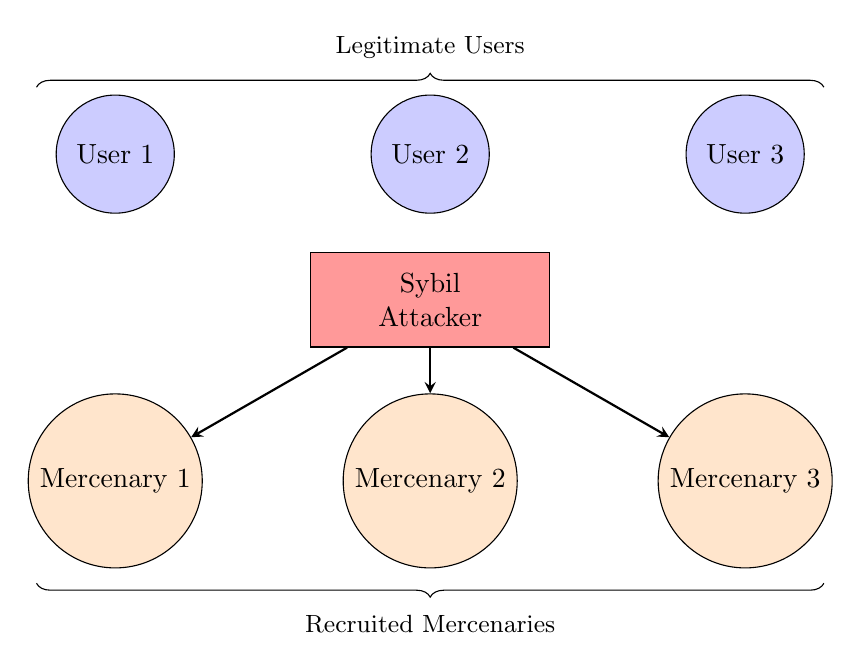
\begin{tikzpicture}[
        node distance=4cm,
        user/.style={circle, draw, fill=blue!20, minimum size=1.5cm},
        mercenary/.style={circle, draw, fill=orange!20, minimum size=1.5cm},
        attacker/.style={rectangle, draw, fill=red!40, minimum width=3cm, minimum height=1.2cm, text width=2.8cm, align=center},
        label/.style={text width=4cm, align=center, font=\small},
        arrow/.style={thick,->,>=stealth}
    ]
        % Main groups
        \node[user] (user1) at (0,4.65) {User 1};
        \node[user] (user2) at (4,4.65) {User 2};
        \node[user] (user3) at (8,4.65) {User 3};
        
        % Attacker
        \node[attacker] (attacker) at (4,2.8) {Sybil\\Attacker};
        
        % Mercenary nodes
        \node[mercenary] (merc1) at (0,0.5) {Mercenary 1};
        \node[mercenary] (merc2) at (4,0.5) {Mercenary 2};
        \node[mercenary] (merc3) at (8,0.5) {Mercenary 3};
        
        % Labels
        \node[label] (legit) at (4,6) {Legitimate Users};
        \node[label] (merc_label) at (4,-1.32) {Recruited Mercenaries};
        
        % Connections
        \draw[arrow] (attacker) -- (merc1);
        \draw[arrow] (attacker) -- (merc2);
        \draw[arrow] (attacker) -- (merc3);
        
        % Grouping brackets
        \draw[decorate,decoration={brace,amplitude=5pt}] (-1,5.5) -- (9,5.5);
        \draw[decorate,decoration={brace,amplitude=5pt,mirror}] (-1,-0.8) -- (9,-0.8);
    \end{tikzpicture}
    \caption{An attacker can recruit humans who are not participating in a network to act as Sybils}
    \label{fig:sybil-attack}
\end{figure}
\vspace{0.1cm}

Soul Bound Tokens (SBTs) are proposed as a potential decentralised identity system, that would be used to ensure individual credentials are not transferable or replicable, and may therefore prove critical in sybil resistance.
However before community recovery mechanisms are broadly adopted by wallet issuers, SBTs are not a complete solution.
In the interim the network may leverage a revocable proto-SBT such as ERC-5484, which maintains the non-transferable and non-replicable properties of an SBT, but allows the token to be burnt under certain conditions \cite{erc5484}.
Sybil resistance must therefore be managed through a layered combination of social and technical mechanisms, including zero-knowledge identity proofs, integrating existing social media account validation, and the use of a reputation system, which can include on-chain activity, repeated engagement and other social signals.

A voice verification network should also support a pseudonymous economy \cite{srinivasan2021psuedonymouseconomy}, whereby users can port their authenticated voice biometrics to a pseudonymous identity they control.
In fact, in order to bootstrap the network, it may not be necessary for voice biometrics to be coupled with a real identity at all.
Such a \textquotesingle training wheels\textquotesingle{} phase---liberated from the need for real identities can enable adoption and stress testing while community wallet recovery mechanisms mature.

\section{Privacy}
\label{sec:results}
Current internet architecture limits privacy, often relying on centralised servers that process and store user data \cite{wang2021cogoverned}.
Privacy for a Voice Verification Network can be maintained by encrypting all biometric and audio data prior to storage in a decentralised cloud network such as IPFS \cite{ipfs2023interplanetary}.

\begin{figure}[H]
    \centering
    \vspace{0.05cm}  % Match spacing with Figure 3
    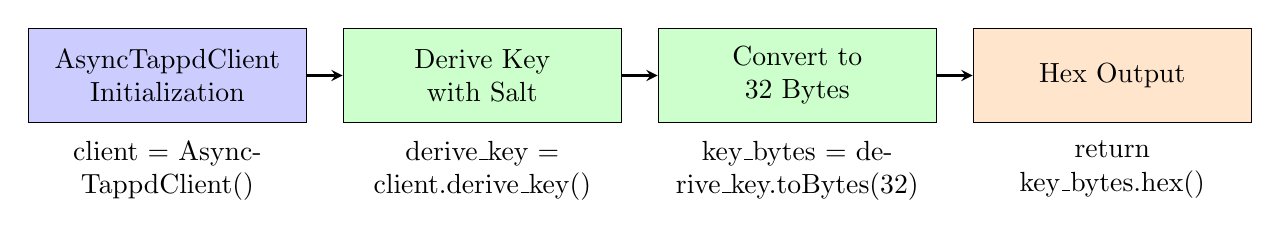
\begin{tikzpicture}[
        node distance=2cm,
        block/.style={rectangle, draw, fill=blue!20, minimum width=3.5cm, minimum height=1.2cm, text width=3.3cm, align=center},
        process/.style={rectangle, draw, fill=green!20, minimum width=3.5cm, minimum height=1.2cm, text width=3.3cm, align=center},
        output/.style={rectangle, draw, fill=orange!20, minimum width=3.5cm, minimum height=1.2cm, text width=3.3cm, align=center},
        arrow/.style={thick,->,>=stealth}
    ]
        % Client initialization
        \node[block] (client) at (0,0) {AsyncTappdClient\\Initialization};
        
        % Key derivation
        \node[process] (derive) at (4,0) {Derive Key\\with Salt};
        
        % Key conversion
        \node[process] (convert) at (8,0) {Convert to\\32 Bytes};
        
        % Final output
        \node[output] (output) at (12,0) {Hex Output};
        
        % Connections
        \draw[arrow] (client) -- (derive);
        \draw[arrow] (derive) -- (convert);
        \draw[arrow] (convert) -- (output);
        
        % Labels with increased vertical spacing
        \node[below=0.1cm of client, text width=3.3cm, align=center] {client = AsyncTappdClient()};
        \node[below=0.1cm of derive, text width=3.3cm, align=center] {derive\_key = client.derive\_key()};
        \node[below=0.1cm of convert, text width=3.3cm, align=center] {key\_bytes = derive\_key.toBytes(32)};
        \node[below=0.1cm of output, text width=3.3cm, align=center] {return key\_bytes.hex()};
    \end{tikzpicture}
    \captionof{figure}{Key derivation process for encryption key generation}
    \label{fig:key-derivation}
\end{figure}
\vspace{0.1cm}

A wallet signature derives a fernet symmetric encryption key \cite{fernet2010fernet} from a Trusted Execution Environment (TEE) network such as Phala \cite{phala2023tee}, making the data undecipherable without key access.

\begin{figure}[H]
    \centering
    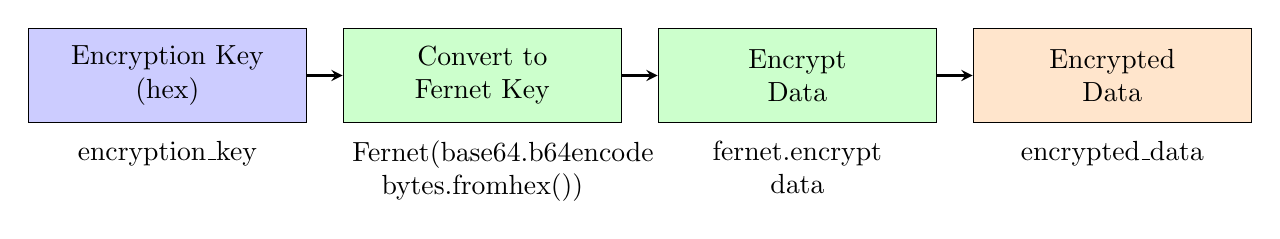
\begin{tikzpicture}[
        node distance=2cm,
        input/.style={rectangle, draw, fill=blue!20, minimum width=3.5cm, minimum height=1.2cm, text width=3.3cm, align=center},
        process/.style={rectangle, draw, fill=green!20, minimum width=3.5cm, minimum height=1.2cm, text width=3.3cm, align=center},
        output/.style={rectangle, draw, fill=orange!20, minimum width=3.5cm, minimum height=1.2cm, text width=3.3cm, align=center},
        arrow/.style={thick,->,>=stealth}
    ]
        % Input key
        \node[input] (key) at (0,0) {Encryption Key\\(hex)};
        
        % Key conversion
        \node[process] (convert) at (4,0) {Convert to\\Fernet Key};
        
        % Encryption
        \node[process] (encrypt) at (8,0) {Encrypt\\Data};
        
        % Final output
        \node[output] (output) at (12,0) {Encrypted\\Data};
        
        % Connections
        \draw[arrow] (key) -- (convert);
        \draw[arrow] (convert) -- (encrypt);
        \draw[arrow] (encrypt) -- (output);
        
        % Labels with two lines
        \node[below=0.1cm of key, text width=3.3cm, align=center] {encryption\_key};
        \node[below=0.1cm of convert, text width=3.3cm, align=center] {Fernet(base64.b64encode\\bytes.fromhex())};
        \node[below=0.1cm of encrypt, text width=3.3cm, align=center] {fernet.encrypt\\data};
        \node[below=0.1cm of output, text width=3.3cm, align=center] {encrypted\_data};
    \end{tikzpicture}
    \captionof{figure}{Fernet encryption process for data protection}
    \label{fig:fernet-encryption}
\end{figure}
\vspace{0.1cm}

A Content Identifier (CID) is generated when the data is stored and this is deployed into a proto-SBT contract issued to the signing wallet.
Only this proto-SBT holding wallet can derive the decryption key from the TEE network.

\begin{figure}[H]
    \centering
    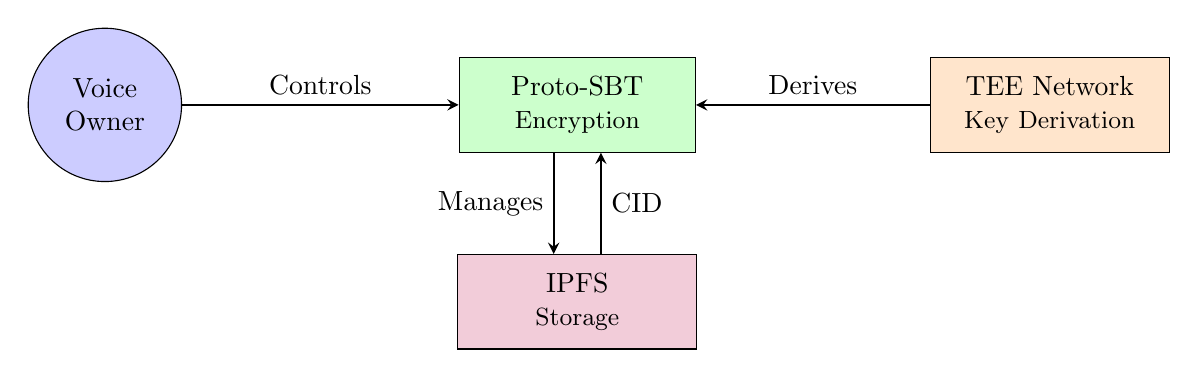
\begin{tikzpicture}[
        node distance=4cm,
        owner/.style={circle, draw, fill=blue!20, minimum size=1.2cm, text width=1.5cm, align=center},
        sbt/.style={rectangle, draw, fill=green!20, minimum width=3cm, minimum height=1.2cm, text width=2cm, align=center},
        tee/.style={rectangle, draw, fill=orange!20, minimum width=3cm, minimum height=1.2cm, text width=2.8cm, align=center},
        ipfs/.style={rectangle, draw, fill=purple!20, minimum width=3cm, minimum height=1.2cm, text width=2.8cm, align=center},
        arrow/.style={thick,->,>=stealth}
    ]
        % Self-custody diagram
        \node[owner] (owner1) at (-6,0) {Voice\\Owner};
        \node[sbt] (sbt1) at (0,0) {Proto-SBT\\\small{Encryption}};
        \node[tee] (tee1) at (6,0) {TEE Network\\\small{Key Derivation}};
        \node[ipfs] (ipfs1) at (0,-2.5) {IPFS\\\small{Storage}};
        
        % Connections for self-custody
        \draw[arrow] (owner1) -- node[above] {Controls} (sbt1);
        \draw[arrow] (tee1) -- node[above] {Derives} (sbt1);
        \draw[arrow] ([xshift=-0.3cm]sbt1.south) -- node[left] {Manages} ([xshift=-0.3cm]ipfs1.north);
        \draw[arrow] ([xshift=0.3cm]ipfs1.north) -- node[right] {CID} ([xshift=0.3cm]sbt1.south);
    \end{tikzpicture}
    \caption{Self-custody solution for voice data management}
    \label{fig:self-custody}
\end{figure}
\vspace{0.1cm}

\section{Intellectual Property, Sovereignty and Custody}
\label{sec:conclusion}
The unique physiological properties of a voice cannot be understood as Intellectual Property (IP) in a traditional sense, and are not protected by existing IP laws.
Though legislation such as the Ensuring Likeness Voice Image Security (ELVIS) Act \cite{elvis2024act} has been signed into law in Tennessee, US, and bills are proposed across the US and other jurisdictions, the ELVIS Act is merely an expansion of \textit{publicity} rights of the voice as "a sound attributable to a particular individual, regardless of whether it contains the actual voice or a simulation" and only applies to unauthorised \textit{commercial} use.
This makes sense, as the voice is a natural biological property of an individual, it is not a product of human invention, however when commercialised a voice being purveyed in a new work can have attributes that allow it to fit into an IP regime, therefore elements of proposed legislation are concerned with making AI voice models licensable.
The No Artificial Intelligence Fake Replicas And Unauthorized Duplications (No AI FRAUD) Act \cite{noaifraud2024act} proposed in the US House of Representatives would "recognize that every individual has a property right in their own likeness and voice, akin to other forms of IP rights\cite{ipwatchdog2024noaifraud}" and the Nurture Originals, Foster Art and Keep Entertainment Safe (NO FAKES) Act \cite{nofakes2024act} introduced in both the US Senate and House of Representatives would grant "each individual or right holder the right to authorize the use of their voice or visual likeness in a digital replica, which the bill states is a property right" \cite{ipupdate2024nofakes}.
Though the scope of these proposals targets broad protection for individuals, as well as outlining the commercial terms for licensing, in practice enforcement is likely to be difficult for anyone other than the corporations that rely on IP as a product.

A voice verification network should exist independently of any IP regime, and not be encumbered by politically or commercially vulnerable legislation.
A voice verification network should be sovereign, enabling the user to own and control their data, and to enable it to be used as they see fit.
This work proposes cryptographic, rather than legal controls, to maintain the integrity of the network, and to ensure that the user's data is not used for purposes other than those intended.
It however may be utilised by nation states to uphold their laws and protect their citizens from deepfake fraud.
Voice data custody solutions may be necessary to support a broader rollout, and data custodians may serve as a bridge between the network and voice owner.

\begin{figure}[H]
    \centering
    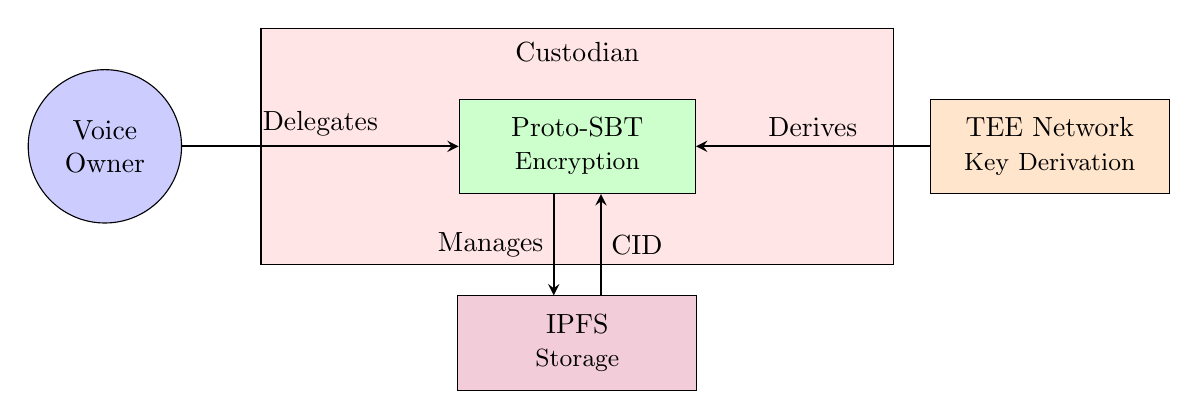
\begin{tikzpicture}[
        node distance=4cm,
        owner/.style={circle, draw, fill=blue!20, minimum size=1.2cm, text width=1.5cm, align=center},
        sbt/.style={rectangle, draw, fill=green!20, minimum width=3cm, minimum height=1.2cm, text width=2cm, align=center},
        tee/.style={rectangle, draw, fill=orange!20, minimum width=3cm, minimum height=1.2cm, text width=2.8cm, align=center},
        ipfs/.style={rectangle, draw, fill=purple!20, minimum width=3cm, minimum height=1.2cm, text width=2.8cm, align=center},
        arrow/.style={thick,->,>=stealth}
    ]
        % Custodial diagram
        \node[above=0.5cm] at (0,0) {\textbf{Custodial}};
        \node[rectangle, draw, fill=red!10, minimum width=8cm, minimum height=3cm, text width=7.8cm, align=center] (custodian) at (0,0.0) {};
        \node[text width=7.8cm, align=center] at (0,1.2) {Custodian};
        \node[owner] (owner2) at (-6,0) {Voice\\Owner};
        \node[sbt] (sbt2) at (0,0) {Proto-SBT\\\small{Encryption}};
        \node[tee] (tee2) at (6,0) {TEE Network\\\small{Key Derivation}};
        \node[ipfs] (ipfs2) at (0,-2.5) {IPFS\\\small{Storage}};
        
        % Connections for custodial
        \draw[arrow] (owner2) -- node[above] {Delegates} (sbt2);
        \draw[arrow] (tee2) -- node[above] {Derives} (sbt2);
        \draw[arrow] ([xshift=-0.3cm]sbt2.south) -- node[left] {Manages} ([xshift=-0.3cm]ipfs2.north);
        \draw[arrow] ([xshift=0.3cm]ipfs2.north) -- node[right] {CID} ([xshift=0.3cm]sbt2.south);
    \end{tikzpicture}
    \caption{Custodial solution for voice data management}
    \label{fig:custodial}
\end{figure}
\vspace{0.1cm}

Custodial solutions are often used in the cryptocurrency space, while self-custody is available to users who wish to administer their cryptographic assets independently of any third party.

\section{AI Voice Agents}
\label{sec:discussion}

Network participants are able to provide their voice to an AI voice agent, which can be used to provide a voice-based service.
The voice model can be provided \textquotesingle as-is\textquotesingle{} or in combination with other voices and sources to create unique voices.
For example, a voice agent could be deployed in a reader app, a chatbot, or a voice assistant, and paid for with royalties issued in a native token representing the individual voice.
Such an AI voice agent marketplace would provide an incentive for users to provide their voice data to the network, and to maintain it over time.

\begin{figure}[H]
    \centering
    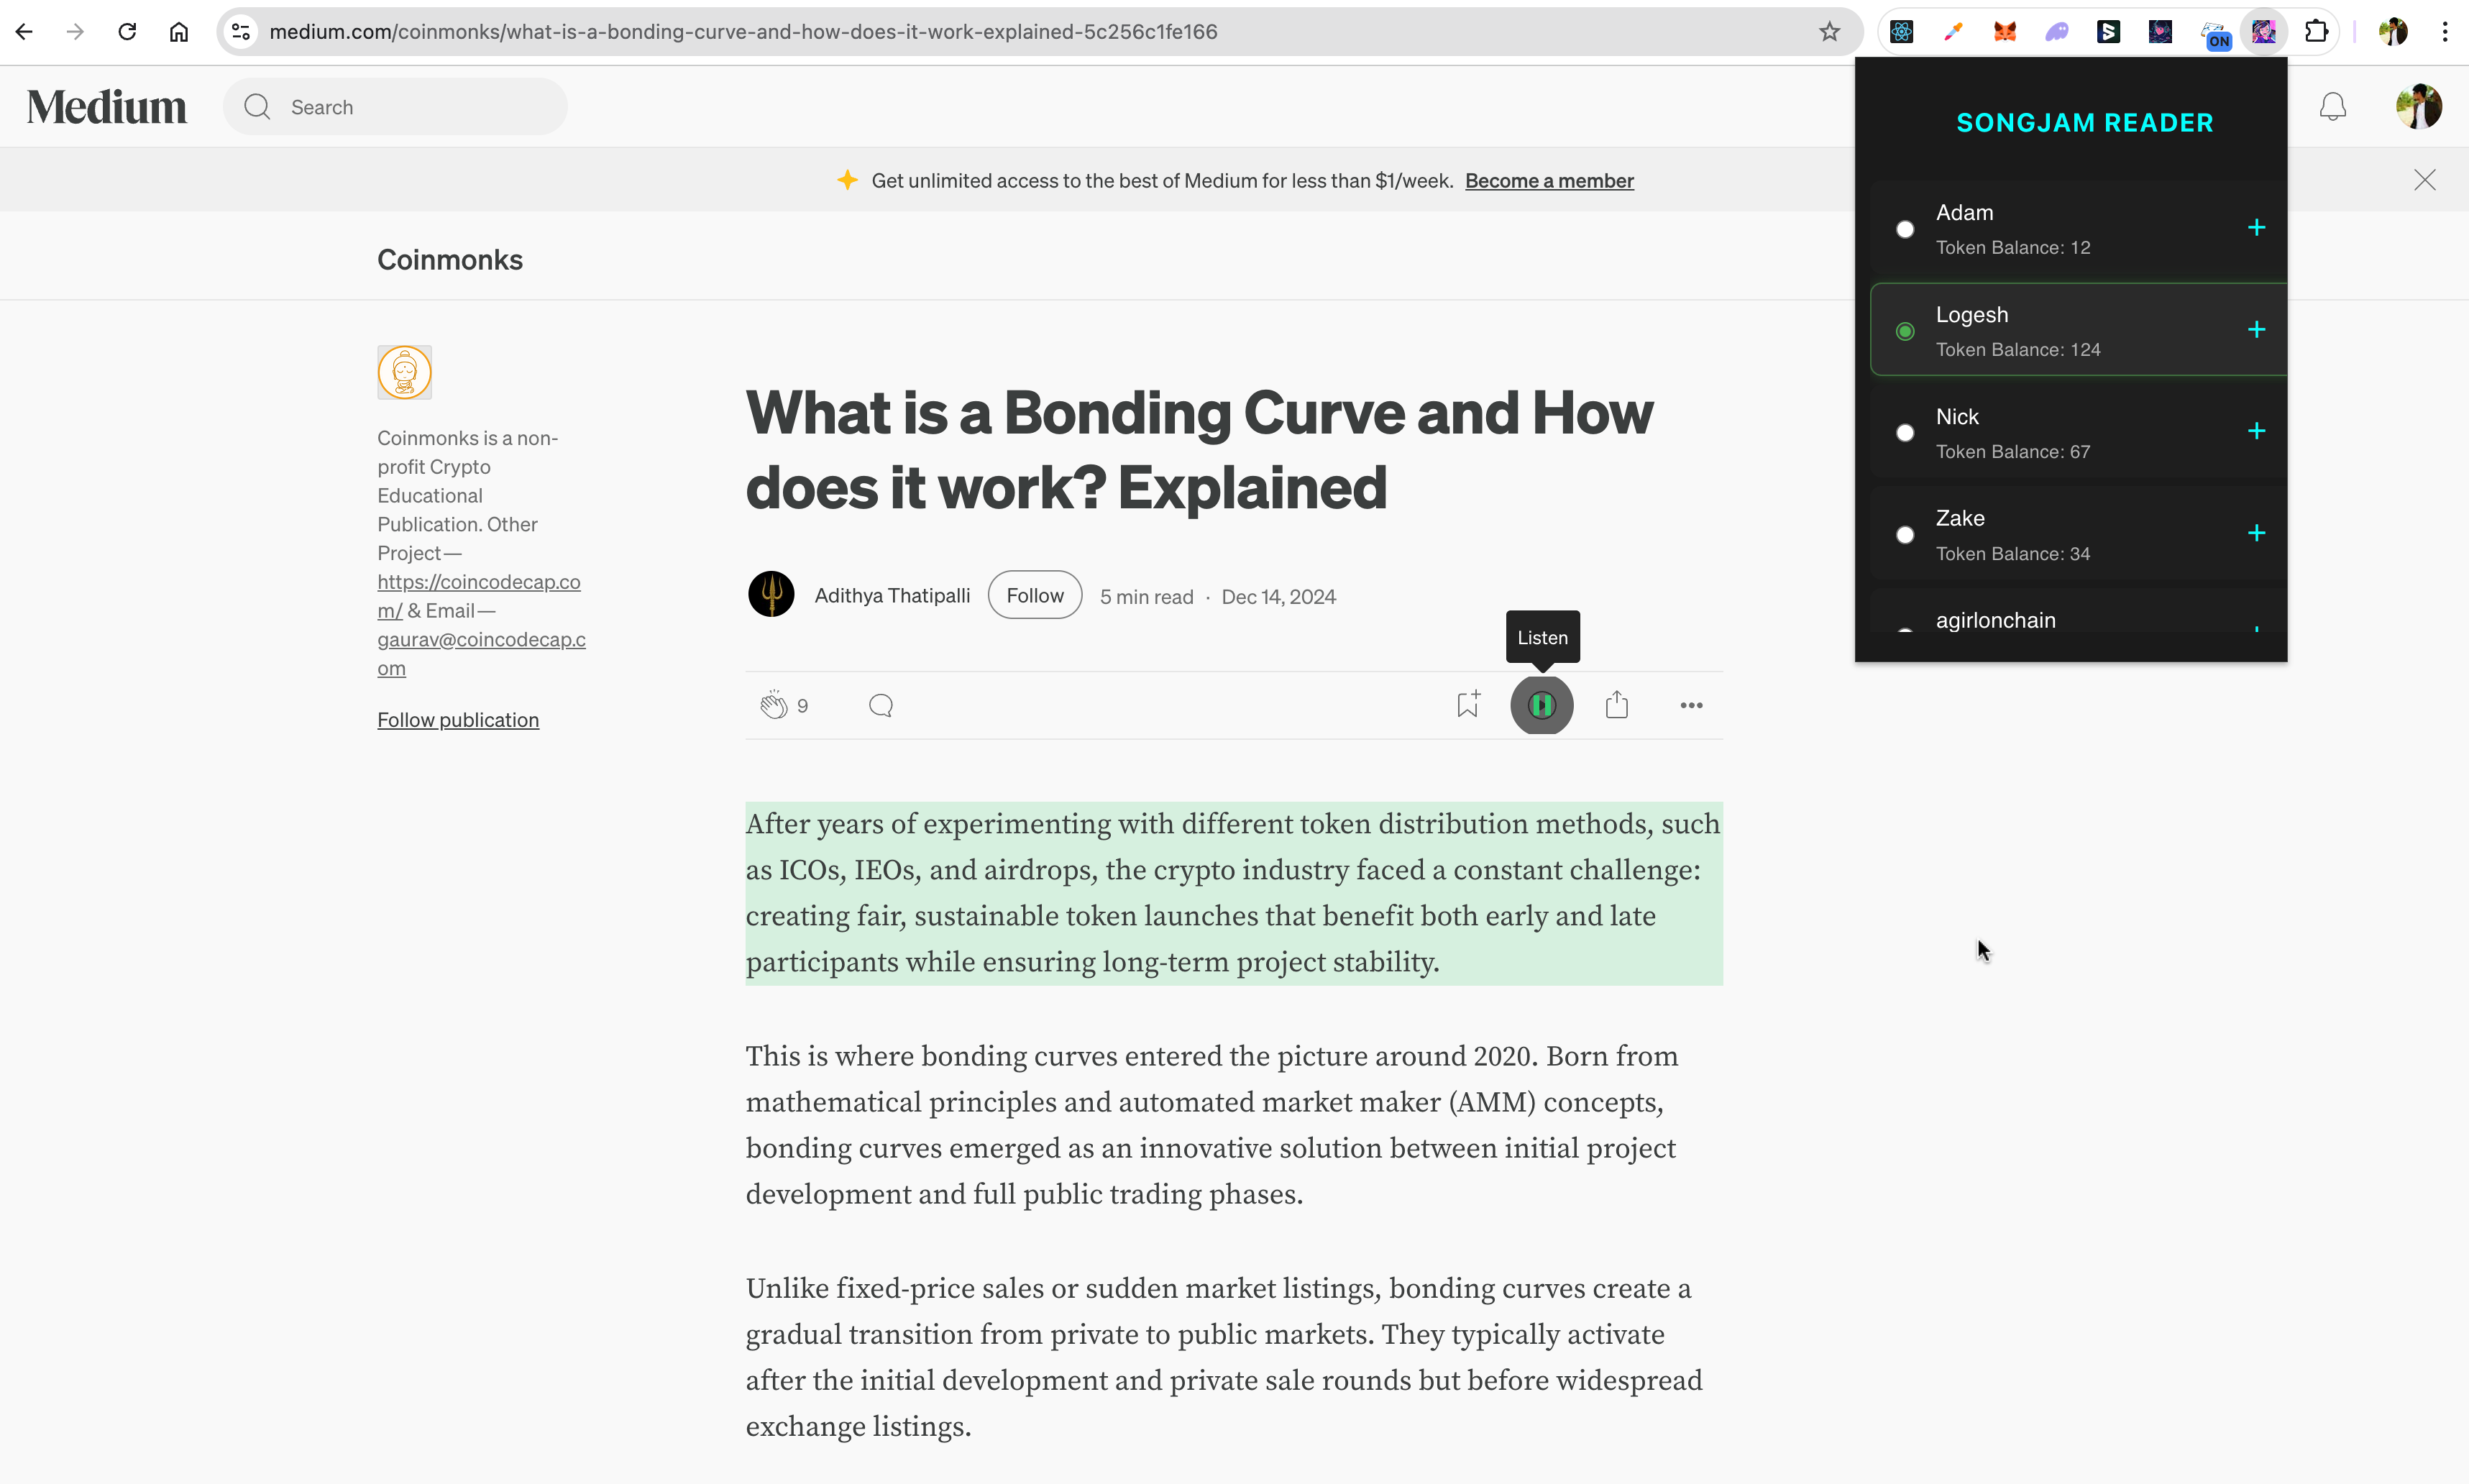
\includegraphics[width=0.8\textwidth]{reader.png}
    \caption{Voice agents deployed in a reader browser extension, displaying remaining token balance}
    \label{fig:reader}
\end{figure}

Users stake corresponding tokens to enable use of an agent, which are burnt based on usage:

\begin{equation}
    S_t = S_{t-1} - \sum_{i=1}^{n} \frac{w_i}{W} \quad \text{where } S_t \geq 0
\end{equation}

Where $S_t$ is the remaining stake at time $t$, $w_i$ is the number of tokens spoken by the AI model for utterance $i$, and $W$ is the total number of tokens in the model's vocabulary. This ensures that one staked token is burnt for each token spoken by the AI voice agent, with partial tokens being accumulated until they sum to a whole token.

Another early use-case sees users spinning-up their own voice agent once they have recorded a sufficient amount of voice data, and deploying it inside an X (formerly Twitter) Space---interactive live audio conversations which have become popular forums for the cryptocurrency community.
By participating in these X Spaces with AI voice agents trained on their voice data and personality, they can grow their X following, expanding their reach and earning potential.

An AI voice agent marketplace can be introduced through the Songjam agentic CRM, an existing platform designed to support growth and analytics for X users by automating processes such as direct messaging, tracking listener data and Automatic Speech Recognition (ASR) with an emphasis on X Spaces.

\begin{figure}[H]
    \centering
    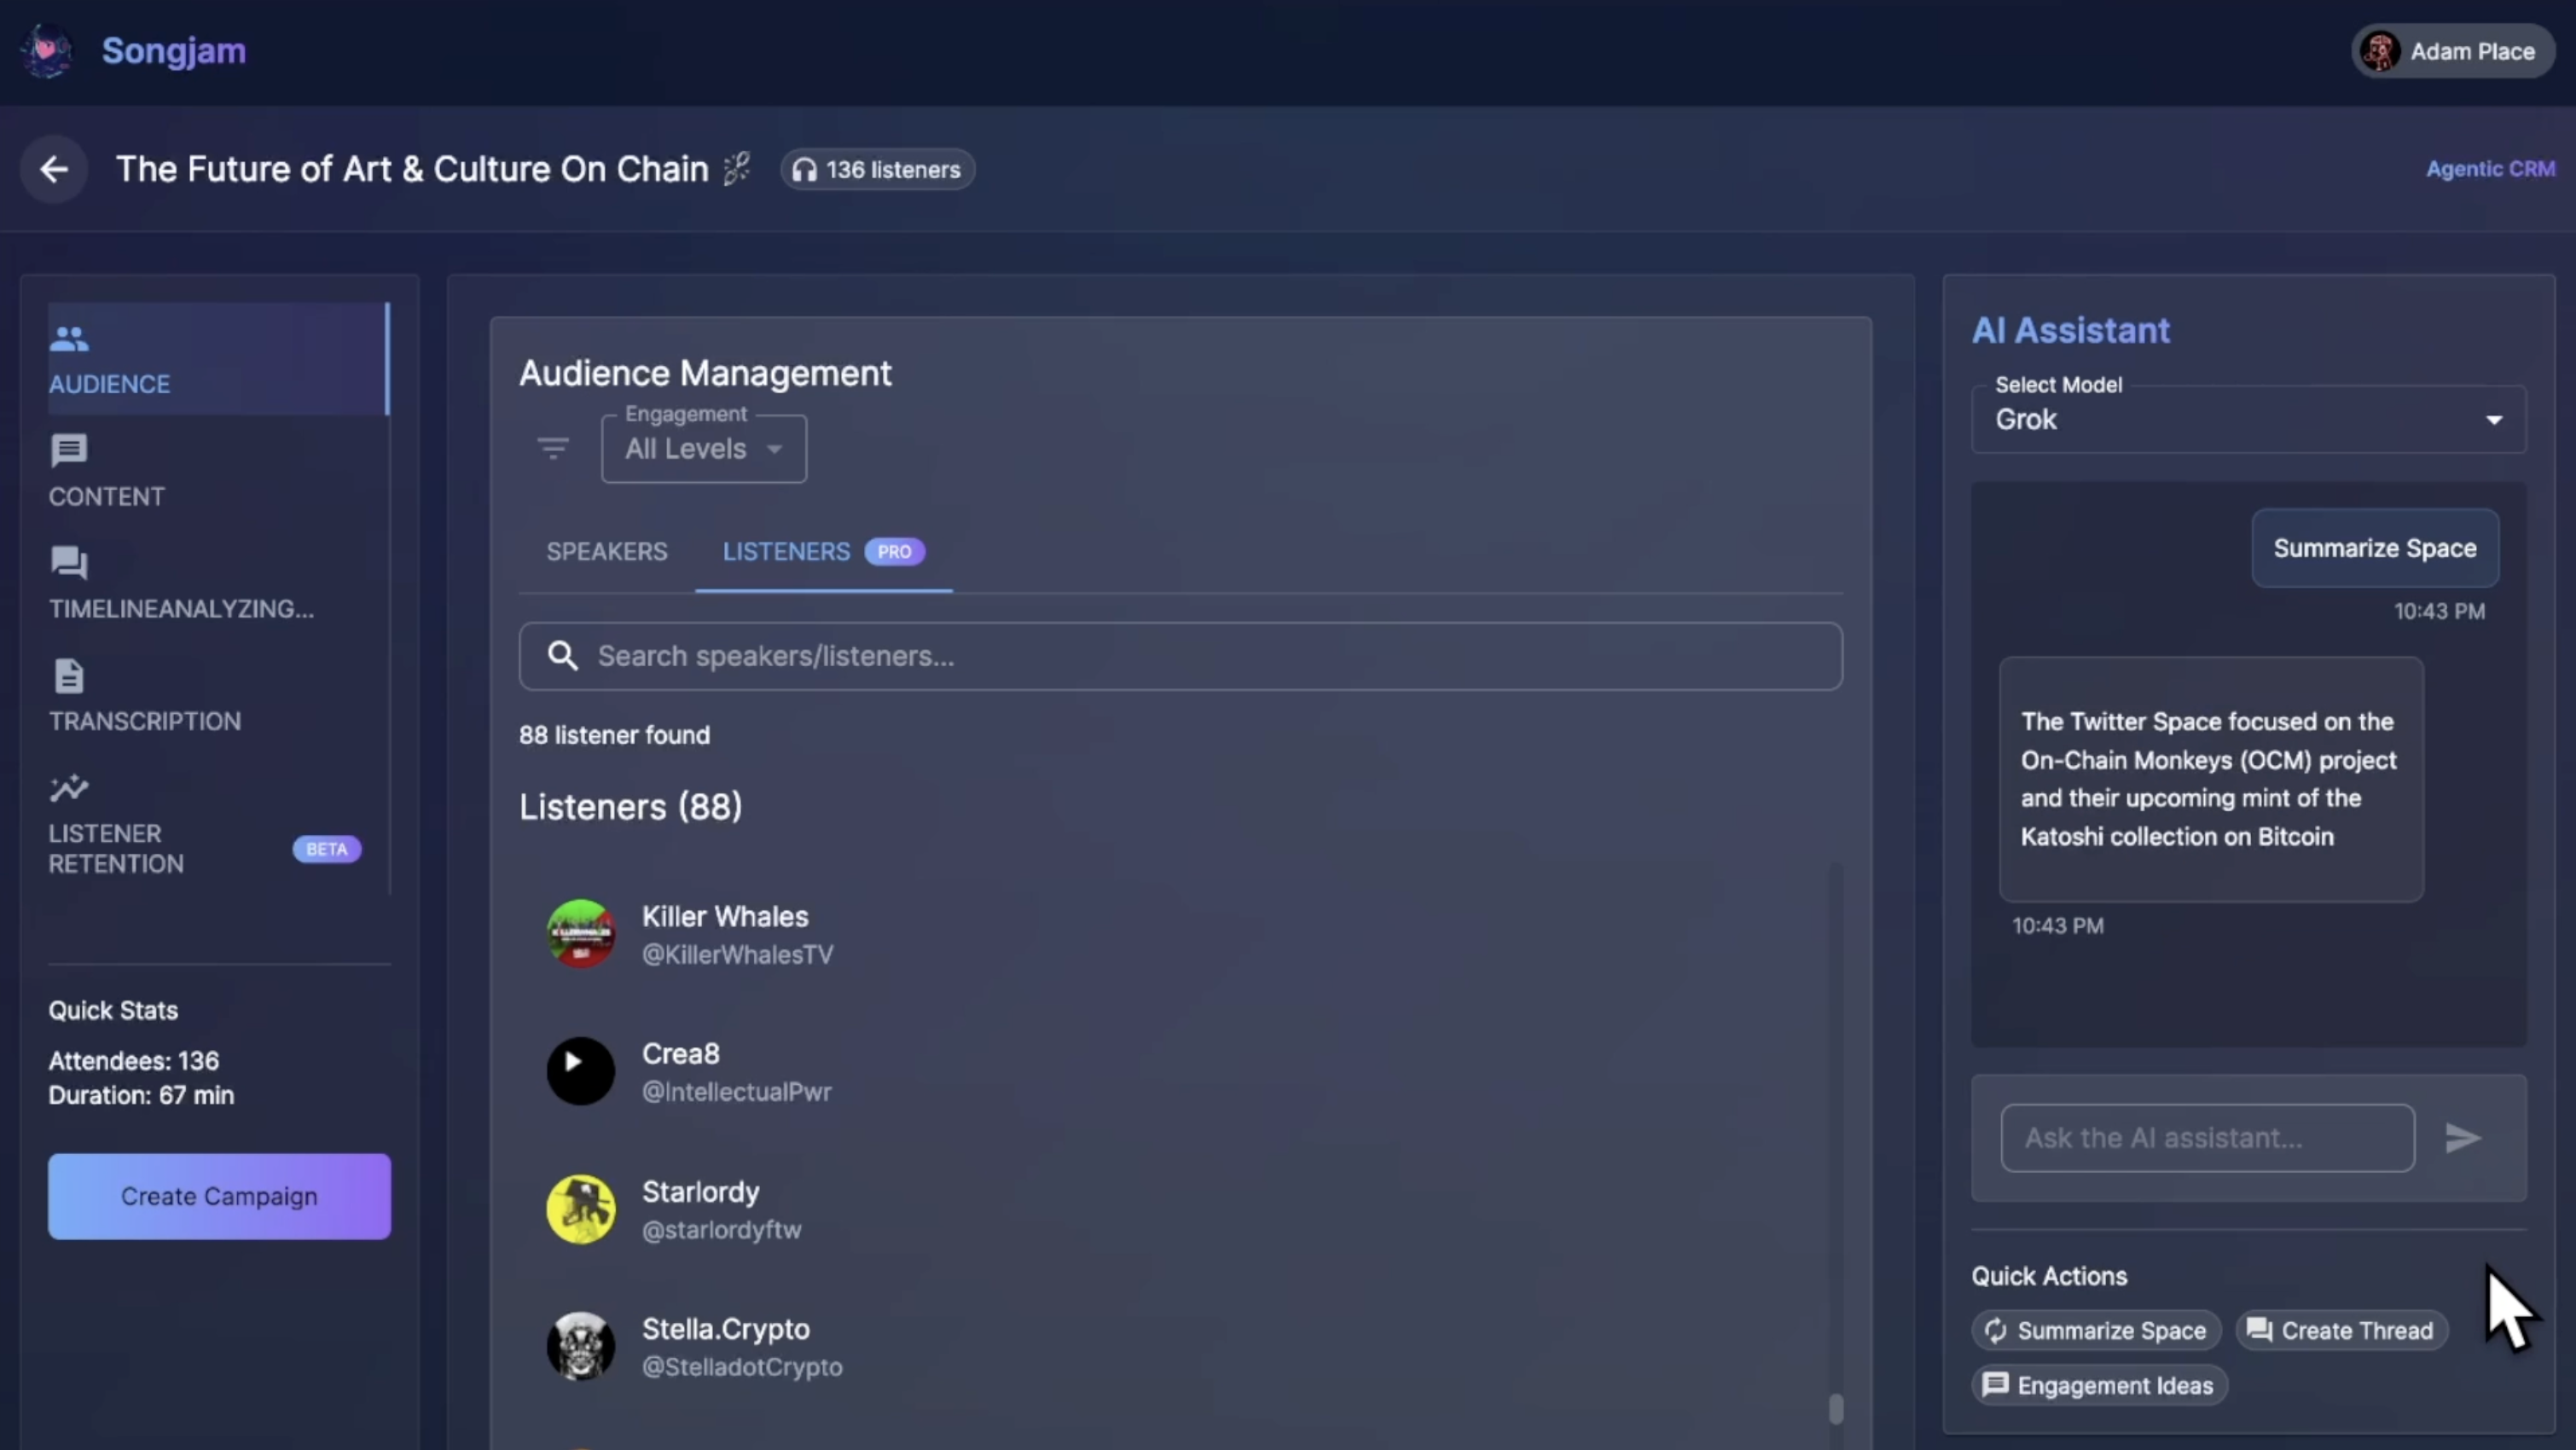
\includegraphics[width=0.8\textwidth]{crm.png}
    \caption{Songjam agentic CRM interface for managing X Spaces}
    \label{fig:crm}
\end{figure}

Focusing on an X Spaces native sandbox can encourage users to spin up creative AI voice agents with customisable personalities, using their own voice or a combination of available voices to create unique voice agents with royalties being split between the original voice owner(s) and the agent owner.
As mentioned in section 3, such a \textquotesingle training wheels\textquotesingle{} phase can support early network growth, helping to ensure the network is robust, while providing a platform for users to experiment within the voice agent ecosystem.
There may be several iterations of the voice agent marketplace and its underlying protocol that must be rolled out and stress-tested at scale before a fully decentralised, cryptographically secure voice verification network can reach maturity.

\section{Data}
\label{sec:data}
Retrieval Augmented Generation (RAG) is a data standard which supports context-rich retrieval for AI models such as Large Language Models (LLMs).
It has become a key component of the AI ecosystem, giving LLMs the ability to access and utilise external data sources to enhance their responses.
WavRAG is a framework that integrates audio data into RAG pipelines without requiring an intermediate ASR step, therefore reducing computational overhead, preserving acoustic information and leveraging a unified multimodal knowledge base ideal for voice data.
Despite these advantages, WavRAG is not yet widely adopted, and the extent to which RAG can contribute to the acoustic aspects such as intonation, expressiveness and other voice characteristics essential to AI voice agents has yet to be extensively investigated.

Furthermore, there are limited high-quality emotion datasets available for the training of voice models, and many researchers are resorting to synthetic data generation due to the cost of collecting and annotating real data \cite{yang2025emovoice, wang2025speechdialoguefactory}.
Model collapse is predicted when a model is trained on recursive synthetic data \cite{shumailov2024model}, in other words when a model is trained on data itself generated by a model.
Though there is limited research into voice model degeneration due to these causes, why risk it when X Spaces presents a goldmine of real-world voice data for training and testing?

Incentivising users to annotate and own their voice data can help to address these issues, and can be supported by the network through a voice data marketplace.
Users may not charge the same price for their voice data as they would for their time, particularly when captured in a public forum they participate in for their own professional or personal benefit.

\begin{figure}[H]
    \centering
    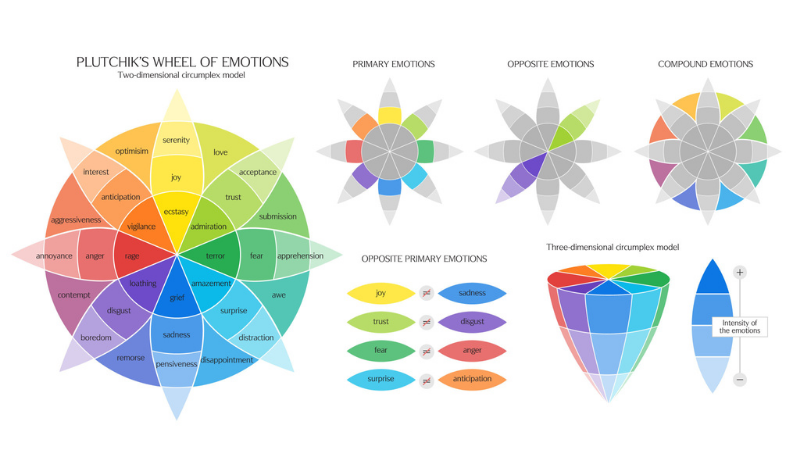
\includegraphics[width=0.8\textwidth]{wheel.png}
    \caption{Plutchik's Wheel of Emotions}
    \label{fig:emotion-wheel-png}
\end{figure}

A speech database can draw from psychologist Robert Plutchik's Wheel of Emotions \cite{plutchik1980general}, which is a model of human emotions based on the theory of psychotherapy.
The wheel is divided into 8 primary emotions, and subsequent sets of secondary and tertiary emotions which represent different levels of intensity, as well as compound emotions.
X Space data is recorded and categorised by the speaker, or other participants in the space including listeners. Metadata is enriched with further context and this forms the foundation of a structured speech dataset.

\begin{figure}[H]
    \centering
    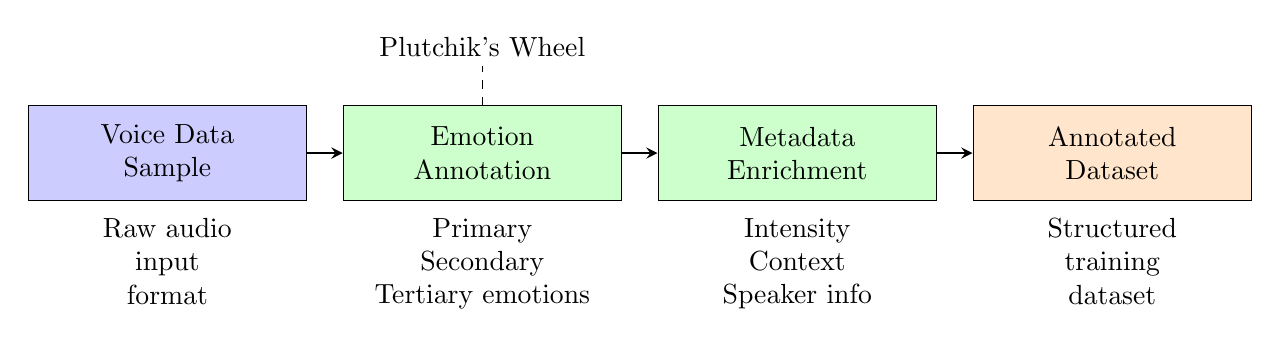
\begin{tikzpicture}[
        node distance=2cm,
        block/.style={rectangle, draw, fill=blue!20, minimum width=3.5cm, minimum height=1.2cm, text width=3.3cm, align=center},
        process/.style={rectangle, draw, fill=green!20, minimum width=3.5cm, minimum height=1.2cm, text width=3.3cm, align=center},
        output/.style={rectangle, draw, fill=orange!20, minimum width=3.5cm, minimum height=1.2cm, text width=3.3cm, align=center},
        arrow/.style={thick,->,>=stealth}
    ]
        % Voice data input
        \node[block] (voice) at (0,0) {Voice Data\\Sample};
        
        % Emotion annotation
        \node[process] (annotate) at (4,0) {Emotion\\Annotation};
        
        % Metadata enrichment
        \node[process] (metadata) at (8,0) {Metadata\\Enrichment};
        
        % Final output
        \node[output] (output) at (12,0) {Annotated\\Dataset};
        
        % Connections
        \draw[arrow] (voice) -- (annotate);
        \draw[arrow] (annotate) -- (metadata);
        \draw[arrow] (metadata) -- (output);
        
        % Labels with three lines
        \node[below=0.1cm of voice, text width=3.3cm, align=center] {Raw audio\\input\\format};
        \node[below=0.1cm of annotate, text width=3.3cm, align=center] {Primary\\Secondary\\Tertiary emotions};
        \node[below=0.1cm of metadata, text width=3.3cm, align=center] {Intensity\\Context\\Speaker info};
        \node[below=0.1cm of output, text width=3.3cm, align=center] {Structured\\training\\dataset};
        
        % Emotion wheel reference
        \node[above=0.5cm of annotate] {Plutchik's Wheel};
        \draw[dashed] (annotate.north) -- ++(0,0.5);
    \end{tikzpicture}
    \caption{Process of annotating voice data using Plutchik's Wheel of Emotions}
    \label{fig:emotion-annotation}
\end{figure}

Making such data available can be defined by the proto-SBT holder, they may wish to keep the data private, give it away for free, monetise it by selling it to be used for training an AI model, or use it for their own voice agent exclusively.
Programmable terms can be used to define the conditions under which the data can be used, and the royalties that are due to the voice owner(s).
Compiling such a structured dataset in a WavRAG pipeline and enabling the network to define its own terms would be a step towards a sovereign open-source AI voice ecosystem.

\section{Conclusion}
\label{sec:conclusion}
This work proposed a cryptographically secure voice verification network, and a framework for the development of an open-source AI voice ecosystem, including a voice agent and voice data marketplace.
Powered by cryptoeconomics and open-source hardware, with demand the network can be bootstrapped rapidly, and scaled to support the needs of the global population.
Leveraging a PoS consensus mechanism, the network is secured through its participants.
The network aims for a future where voice data is owned by the individual, and can be used as they see fit.
Nevertheless, the network may be used in a custodial manner, and data custodians may administer voice data for the benefit of individual voice owners.
This architecture establishes a durable paradigm for voice data security, ensuring persistent user control and safeguarding individual voice assets against emerging threats in an adversarial digital landscape.

Due to the recency of convincing speech synthesis technology there is limited precedent for voice data protection, unlike the incumbent IP administrations which have established practices. This presents a unique opportunity to establish a voice sovereignty standard for the age of AI.
While legal systems take time to adjust across different jurisdictions, a cryptographic voice verification network operating in a decentralised manner---leveraging open-source hardware to address the distribution challenge of proprietary hardware---can be deployed globally and scaled rapidly in alignment with the natural rights of the individual over their own voice.

\bibliographystyle{unsrt} % Changed for debugging
\bibliography{references}

\end{document} 